\documentclass{article}

\usepackage{graphicx}
\usepackage{tikz}
\usepackage{tikzsymbols}
\usetikzlibrary{calc,patterns,shapes.geometric}
\pagestyle{empty}
\usepackage[margin=0pt]{geometry}
\geometry{papersize={14in,12in}}

\def\centerarc[#1](#2)(#3:#4:#5){\draw[#1] ($(#2)+({#5*cos(#3)},{#5*sin(#3)})$) arc (#3:#4:#5);}

\begin{document}
	\begin{figure}
		\centering
		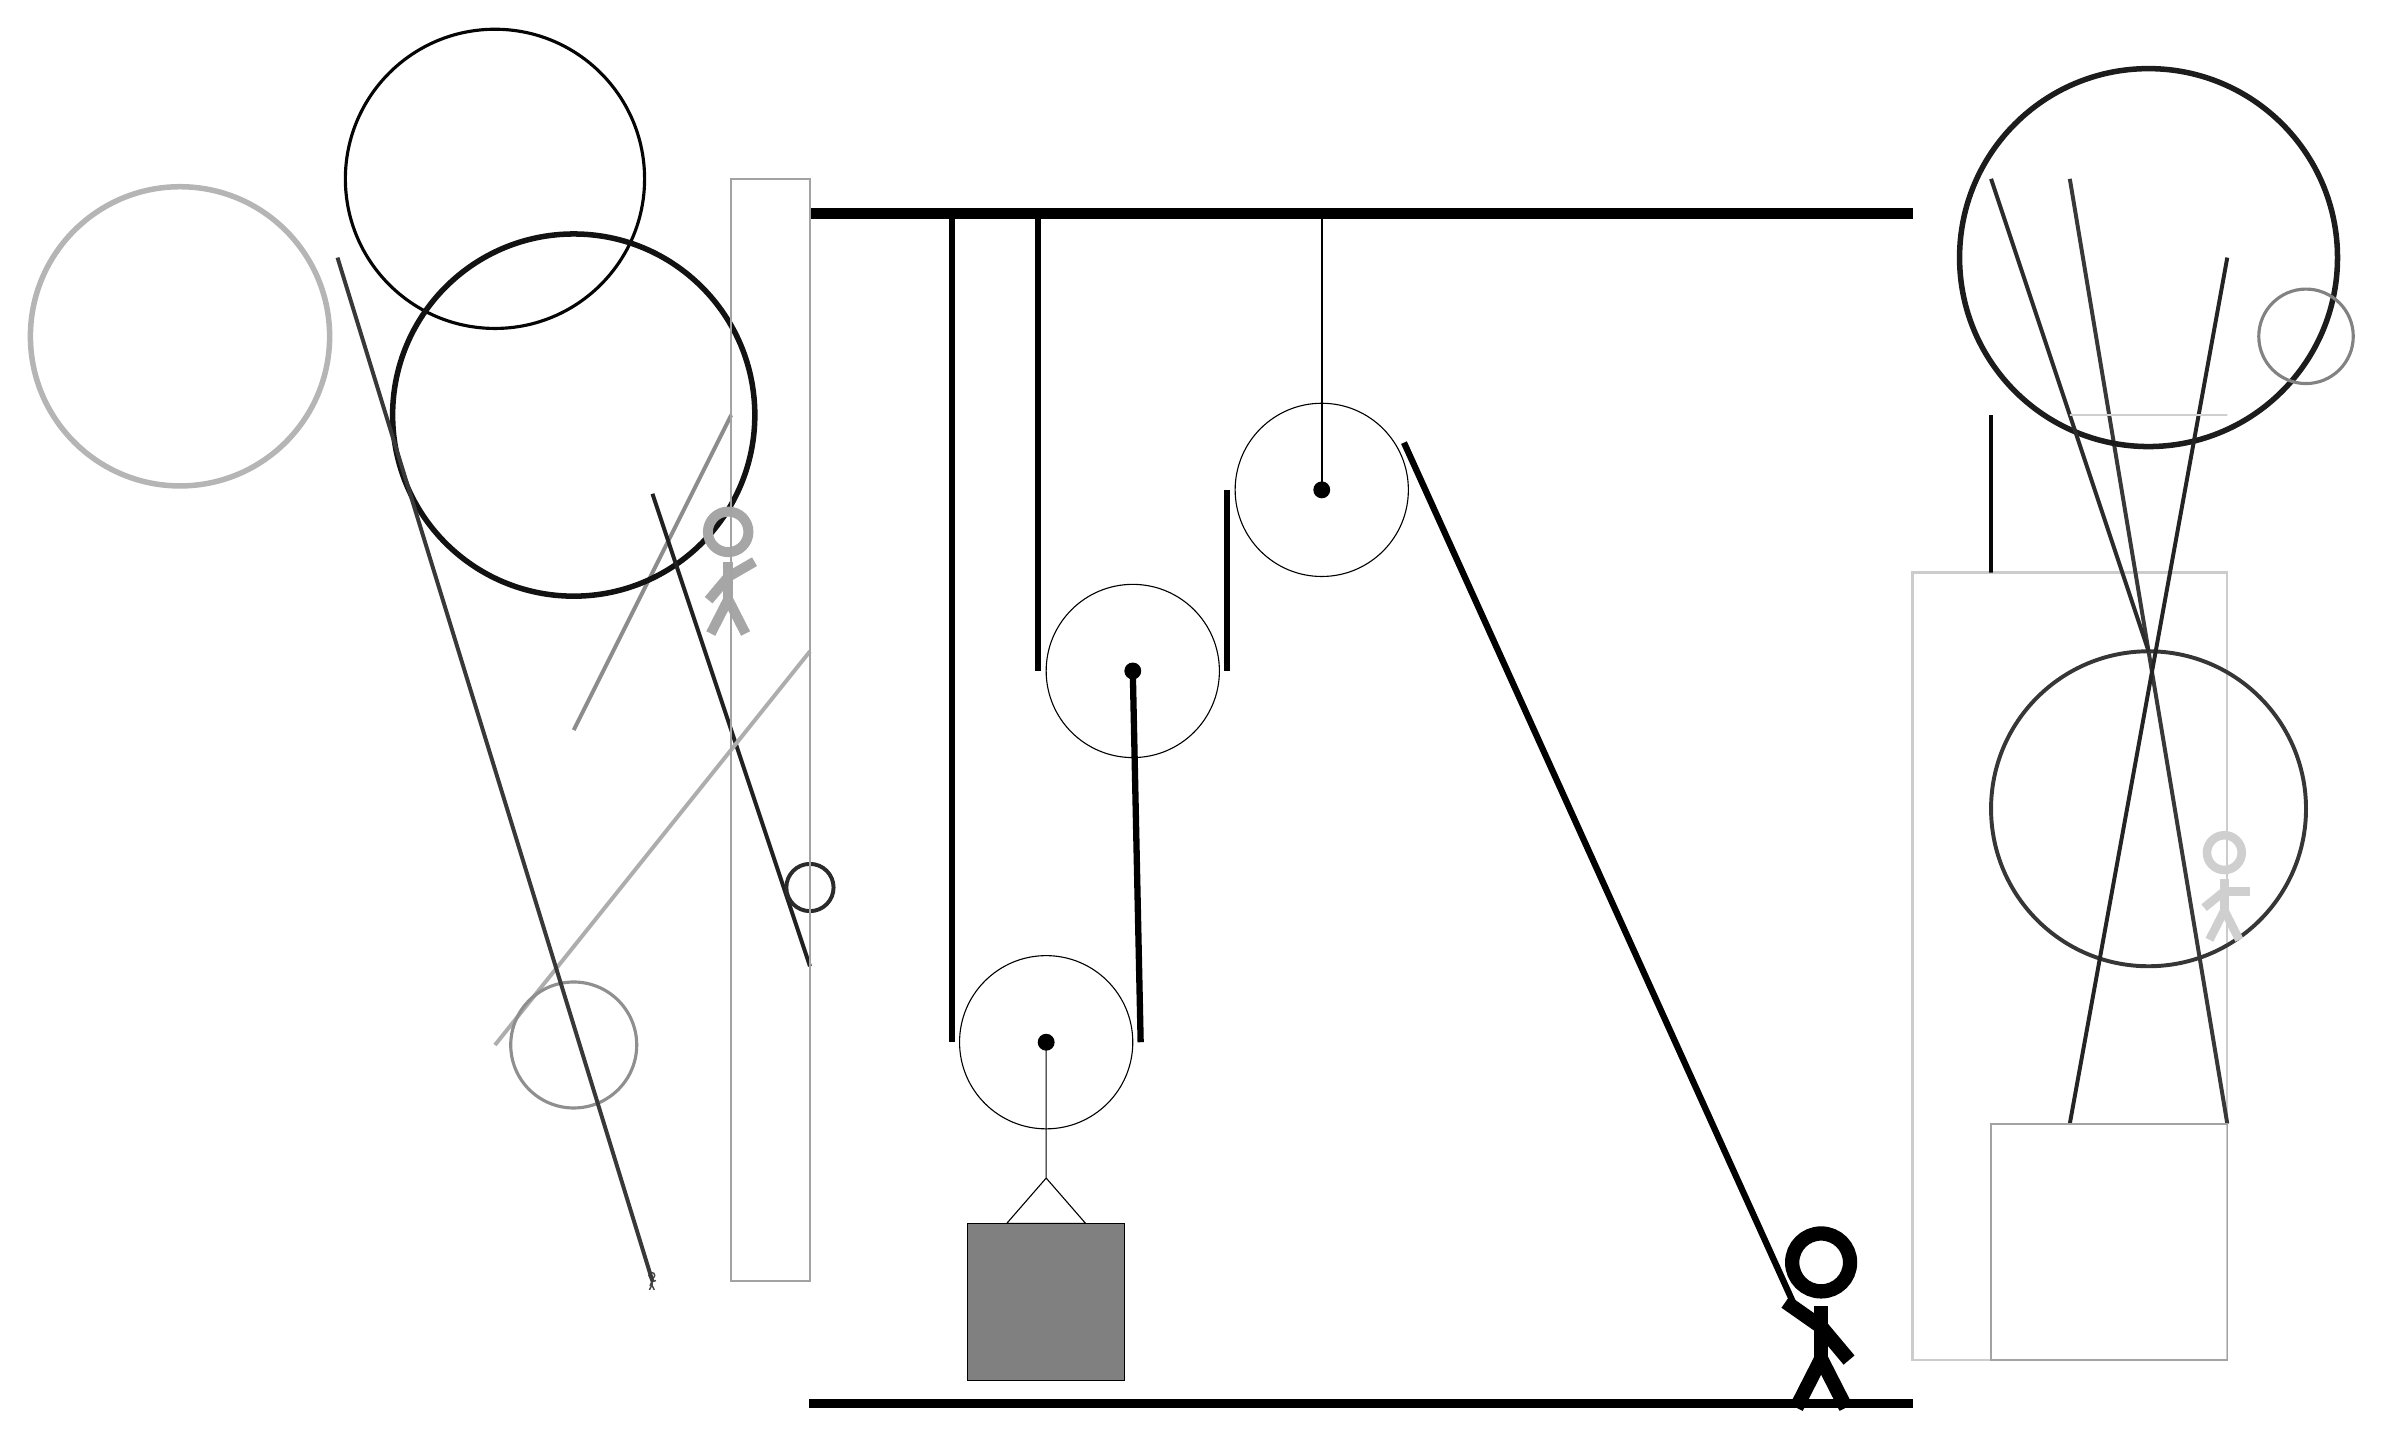
\begin{tikzpicture}
			%%%%% START %%%%%
			
			\draw[fill=black] (-2, 11.5) rectangle (12, 11.625);
			
			\draw (1, 1.035) circle (1.1);
			\draw[fill=black] (1, 1.035) circle (0.1);
			
			\draw (2.1, 5.75) circle (1.1);
			\draw[fill=black] (2.1, 5.75) circle (0.1);
			
			\draw (4.5, 8.05) circle (1.1);
			\draw[fill=black] (4.5, 8.05) circle (0.1);
			\draw[thick] (4.5, 8.05) -- (4.5, 11.5);
			
			\draw (1, 1.035) -- (1, -0.69) -- (0.5, -1.265) -- (1.5, -1.265) -- (1, -0.69);
			\draw[fill=black!50] (0, -1.265) rectangle (2, -3.265);
			
			\draw[line width=0.3mm, color=black!20] (12, 7) rectangle (16, -3);
			
			\draw [line width=0.5mm, color=black!79](15, 4) circle (2.0);
			\draw[line width=0.5mm, color=black!45](-3, 9) -- (-5, 5);
			\draw[line width=0.5mm, color=black!78](14, 12) -- (16, 0);
			\draw [line width=0.7mm, color=black!29](-10, 10) circle (1.9);
			\node[line width=0.5mm, color=black!19] at (16, 3) {\Strichmaxerl[6][39][0]};
			\draw [line width=0.4mm, color=black!98](-6, 12) circle (1.9);
			
			\draw [line width=0.7mm, color=black!93](-5, 9) circle (2.3);
			\draw[line width=0.5mm, color=black!87](-4, 8) -- (-2, 2);
			\draw [line width=0.7mm, color=black!89](15, 11) circle (2.4);
			\draw[line width=0.5mm, color=black!32](-2, 6) -- (-6, 1);
			
			\draw [line width=0.4mm, color=black!44](-5, 1) circle (0.8);
			\node[line width=0.2mm, color=black!35] at (-3, 7) {\Strichmaxerl[7][50][30]};
			
			\node[line width=0.5mm, color=black!73] at (-4, -2) {\Strichmaxerl[1][64][17]};
			\draw[line width=0.5mm, color=black!86](16, 11) -- (14, 0);
			\draw[line width=0.5mm, color=black!83](15, 6) -- (13, 12);
			\draw [line width=0.5mm, color=black!83](-2, 3) circle (0.3);
			
			\draw[line width=0.2mm, color=black!36] (13, -3) rectangle (16, 0);
			\draw[line width=0.5mm, color=black!78](-4, -2) -- (-8, 11);
			\draw [line width=0.4mm, color=black!49](17, 10) circle (0.6);
			\draw[line width=0.2mm, color=black!19] (14, 9) rectangle (16, 9);
			\draw[line width=0.3mm, color=black!36] (-2, 12) rectangle (-3, -2);
			\draw[line width=0.4mm, color=black!97] (13, 9) rectangle (13, 7);
			
			\draw[line width=0.8mm] (-0.2, 11.5) -- (-0.2, 1.035);
			\centerarc[line width=0.8mm](1, 1.035)(180:360:1.2000000000000002);
			\draw[line width=0.8mm](2.2, 1.035) -- (2.1, 5.75);
			\draw[line width=0.8mm] (0.9, 11.5) -- (0.9, 5.75);
			\centerarc[line width=0.8mm](2.1, 5.75)(180:360:1.2000000000000002);
			\draw[line width=0.8mm](3.3, 5.75) -- (3.3, 8.05);
			\centerarc[line width=0.8mm](4.5, 8.05)(30:180:1.2000000000000002);
			\draw[line width=0.8mm] (5.544, 8.65) -- (10.5, -2.3);
			
			\node at (10.8, -2.5) {\Strichmaxerl[10][-35][-50]};
			
			\draw[fill=black] (-2, -3.5) rectangle (12, -3.6);
			
			%%%%% END %%%%%
		\end{tikzpicture}
	\end{figure}	
\end{document}